\documentclass[9pt,twocolumn]{extarticle}
\usepackage[a4paper,top=1.5cm,bottom=1.5cm,left=1.45cm,right=1.45cm,columnsep=0.55cm]{geometry}
\usepackage[T1]{fontenc}
\usepackage[utf8]{inputenc}
\usepackage{mathptmx}
\usepackage{amsmath,amssymb,bm}
\usepackage{booktabs,array,tabularx}
\usepackage{graphicx}
\usepackage{xcolor}
\usepackage[hidelinks]{hyperref}
\usepackage{microtype}
\usepackage{titlesec}
\usepackage{caption}
\usepackage{enumitem}
\usepackage{stfloats}
\captionsetup{font=small,labelfont=bf,skip=3pt}
\titlespacing*{\section}{0pt}{6pt}{2.5pt}
\titleformat{\section}{\normalsize\bfseries}{\thesection}{0.5em}{}
\setlength{\parskip}{0pt}
\setlength{\parindent}{1.1em}
\setlist{nosep,leftmargin=1.2em}
\setlength{\abovedisplayskip}{3pt}\setlength{\belowdisplayskip}{3pt}
\setlength{\abovedisplayshortskip}{2pt}\setlength{\belowdisplayshortskip}{2pt}
\setlength{\textfloatsep}{7pt}\setlength{\floatsep}{5pt}\setlength{\intextsep}{5pt}
\newcommand{\code}[1]{\texttt{\small #1}}
\newcolumntype{Y}{>{\raggedright\arraybackslash}X}

\title{\vspace{-1.6em}\Large\bfseries Spending Fewer Atoms: Slack-Free One-Hot Clustering of the Capacitated Vehicle Routing Problem on an Analog Neutral-Atom Register}
\author{\normalsize Team Qualies --- DuQuantum Hackathon, Pasqal challenge (Track A primary, Track B supplementary)}
\date{\normalsize 25 October 2026 \quad$\cdot$\quad repository \code{qhack/} (one-command reproduction: \code{python scripts/make.py demo})}

\begin{document}
\maketitle
\vspace{-1.4em}

\noindent\textbf{Abstract.}
We put the clustering half of the capacitated vehicle routing problem (CVRP) onto Pasqal's \code{AnalogDevice} with \emph{no slack atoms at all}. Customers are assigned to vehicles with one-hot variables; the capacity inequality is handled by unbalanced penalization, which on one-hot strings collapses exactly to a load-balance coupling. Every coupling is positive and every linear term is equal, so the model runs on a single global detuning with $NK$ atoms: 8, 30 and 60 on tiers S, M and L, against 14, 45 and 80 for the textbook slack encoding. The report is organised around the chain of improvements that took this model from paper to a working register. A structure-aware embedder---rigid 5\,\textmu m polygons fitted on the one-hot subspace---raised the probability that a raw shot is the model-optimal clustering from 3--13\,\% to 62--90\,\%, and a pulse scan raised it further to \textbf{89--99\,\% on all five tier-S instances}, with feasibility 0.95--1.00. On larger registers we derived and enforced a physical bound on the final detuning, which took tier M from 0\,\% to 98--100\,\% decodable shots, and matched the register geometry and drive to the $K=4$ energy scale, which took tier L from under 1\,\% to \textbf{14--23\,\% capacity-feasible shots}. Every gap is computed on feasible decodes only, and everything that did not work is listed.

\section{What we built}
\begin{itemize}
\item \textbf{A slack-free model} (Sec.~\ref{sec:model}): one-hot assignment plus unbalanced penalization; the \emph{one-hot identity} removes every non-uniform linear term exactly. 25\,\% of the atom budget saved on L.
\item \textbf{A structure-aware embedder} (Sec.~\ref{sec:embed}): it asks the register to reproduce only what the model needs on valid strings, not every pairwise coupling.
\item \textbf{Two derived physical bounds} for one-hot cliques on a planar register, $\delta_f<U_{\min}$ and the $1/8$ coupling collapse of a $K=4$ square, each turned into a code rule.
\item \textbf{A reproducible pipeline}: seeded, certified instances; exact references; committed registers; Pulser-validated sequences; four emulators cross-checked; 79 result rows; plus two verified routing encodings for Track B.
\end{itemize}

\section{Problem and decomposition (Derive 2.1)}
Customers $i\in C=\{0,\dots,N-1\}$ have locations $p_i\in[0,100]^2$ and integer demands $d_i$. There are $K$ identical vehicles of capacity $Q$ and a depot fixed at the centre $(50,50)$ before clustering; travel costs $c_{uv}$ are Euclidean. A valid plan puts every customer on exactly one vehicle (an \textbf{equality}), loads no vehicle beyond $Q$ (an \textbf{inequality}), and orders each vehicle's visits; we minimise total distance, and an unused vehicle costs nothing. Encoding vehicle \emph{and} visit order needs $\sim N^2K$ binaries (32/300/900), so we use cluster-first/route-second: the register decides which customers share a vehicle, and each cluster is routed by exact Held--Karp. The price is the \emph{decomposition gap}, which we report on every instance.

\section{What the register minimises (Derive 3.1)}
At the end of the pulse $\Omega=0$, so the device Hamiltonian is diagonal and assigns each bitstring $x$ the cost
\begin{equation}
E_{\rm dev}(x)= -\delta_f\sum_i x_i+\sum_{i<j}\frac{C_6}{r_{ij}^6}\,x_ix_j .
\label{eq:dev}
\end{equation}
This is a QUBO with three built-in rules. The \textbf{laser} sets one linear coefficient, $-\delta_f$, shared by every atom ($|\delta|\le125.66$\,rad/\textmu s). The \textbf{positions} set every coupling, all positive, at most $C_6/(5\,\text{\textmu m})^6=55.4$\,rad/\textmu s and never exactly zero. $C_6$ is fixed physics. So any model we run must have uniform linear terms and positive couplings.

\section{The model (A1): one-hot, no slack}\label{sec:model}
\textbf{Variables.} $x_{ik}=1$ iff customer $i$ rides on vehicle $k$; $NK$ binaries and nothing else.
\textbf{Objective.} Total pairwise distance inside each cluster, $f(x)=\sum_k\sum_{i<j}d_{ij}x_{ik}x_{jk}$: quadratic, positive, and additive over clusters, so an exact set-partition dynamic programme certifies the model optimum on every tier.
\textbf{Exactly-one.} The penalty $A\sum_i(1-\sum_kx_{ik})^2$ expands to a linear term $-A$ on every bit and a coupling $+2A$ between the $K$ bits of each customer.
\textbf{Capacity.} With slack $g_k=Q-L_k\ge0$, $L_k=\sum_id_ix_{ik}$, unbalanced penalization \cite{montanez} adds $\sum_k[-\lambda_1g_k+\lambda_2g_k^2]$ and needs no auxiliary bits. Its linear part is $\sum_ic_i\sum_kx_{ik}$ with $c_i=d_i(\lambda_1-2\lambda_2Q+\lambda_2d_i)$. On every one-hot string $\sum_kx_{ik}=1$, so this part equals the constant $\sum_ic_i$. We call this \emph{the one-hot identity}: it lets us drop every non-uniform linear term, and $\lambda_1$ with it, without changing the model where it lives. What remains is
\begin{equation}
2\lambda_2\sum_k\sum_{i<j}d_id_j\,x_{ik}x_{jk}=\lambda_2\sum_kL_k^2+\text{const},
\end{equation}
a soft load-balance term. The final cost is
\begin{equation}
E(x)=\sum_k\sum_{i<j}w_{ij}x_{ik}x_{jk}+A\sum_i\Big(1-\sum_kx_{ik}\Big)^2,\;\; w_{ij}=d_{ij}+2\lambda_2d_id_j ,
\end{equation}
with all couplings positive and all linear terms $-A$, so $\delta_f=\alpha A$ realises it with no DMM.
\textbf{Weights.} $A=\max_i\sum_{j\ne i}w_{ij}+1$ provably makes every global minimiser one-hot. $\lambda_2=\kappa R/(2Q)$, $R=\max_i\sum_jd_{ij}$, $\kappa=0.15$, chosen by brute force on 40 toy seeds and verified on all five shipped S instances. Because capacity is soft, \emph{we score only feasible decodes} and always report the feasibility rate.

\begin{table}[t]\centering\small
\caption{Variable count (Derive 4.1), generated by \code{scripts/variable\_count.py}; $B=\lceil\log_2(Q{+}1)\rceil$ slack bits per vehicle.}
\begin{tabular}{@{}lcccc@{}}\toprule
Encoding & S & M & L & fits 80? \\\midrule
Assignment only ($NK$) & 8 & 30 & 60 & yes \\
+ binary slack ($NK+KB$) & 14 & 45 & 80 & yes (L = cap) \\
\textbf{Ours, \code{onehot-ub} ($NK$)} & \textbf{8} & \textbf{30} & \textbf{60} & \textbf{yes} \\\bottomrule
\end{tabular}
\label{tab:vars}
\end{table}

\textbf{Cost (Table~\ref{tab:vars}).} We save 6/15/20 atoms and never read out a bit we throw away. The real cost is geometric: a customer's $K$ atoms must sit 5\,\textmu m apart, so every other atom is almost equidistant from them, and couplings meant to be zero come out as large as the wanted ones. Section~\ref{sec:embed} is our answer.

\section{Instances (A2) and references}
A seeded generator draws a balanced assignment \emph{first} and then demands that fit each vehicle's remaining capacity, so every instance is feasible by construction. That assignment ships as the certificate; \code{cvrp.validator} regenerates each instance from its seed and re-checks it. We use S seeds 0--4 and M, L seeds 0--2, with load ratios $\rho$ = 0.64--0.86 / 0.70--0.95 / 0.60--0.71 and $d_{\max}/Q$ = 0.43--0.57 / 0.40 / 0.30--0.33. \textbf{References} follow brief Sec.~9.3. CPLEX could not be installed, so $C^*$ is the best of \code{qubo-solver}'s simulated annealing on our QUBO and a constrained annealer on the CVRP (10 seeded restarts each, 60\,s limit, parameters in each instance file). On tier S an exhaustive search agrees 5/5, so those are \emph{proven optima}; M and L are \emph{best known}.

\section{Embedding (A3): ask the register for less}\label{sec:embed}
\textbf{Where we started.} A generic least-squares placement of the coupling graph gave a relative coupling error $\|U/\alpha-J\|_F/\|J\|_F$ of 0.95, and on S\_seed04 the register's own ground state was an infeasible string.

\textbf{The idea.} The model only lives on one-hot strings, where each pair of customers contributes exactly one coupling. So the cross-vehicle couplings do not have to vanish; they only have to be constant. Only the \emph{effective} coupling $U(i,k;j,k)-\overline{U(i,k;j,l\ne k)}$ must equal $\alpha w_{ij}$.

\textbf{The embedder} (\code{cvrp/embed\_onehot.py}) makes each customer a rigid regular $K$-gon of side 5\,\textmu m, which realises the exactly-one clique exactly. It then fits only the polygon centres and orientations so that the device energies of all one-hot strings match $\alpha E_{\rm QUBO}$, keeps every single-flip defect above its parent, and fits $\delta_f$ as a free parameter. Registers are cached and committed so every row is reproducible. On tier S the full-matrix error falls to 0.21--0.32, and the register's own ground state \emph{is} the model optimum on 5/5 instances (Fig.~\ref{fig:emb}a).

\textbf{Two bounds we derived and enforced.} In an isolated $K$-gon, one excitation beats two only if $0<\delta_f<U_{\min}$, where $U_{\min}$ is the \emph{weakest} coupling inside the polygon. For $K\le3$ that is 55.1\,rad/\textmu s, and tier S fits land at 35--38. On tier M the fit ran to the device maximum, 125.66\,rad/\textmu s, and \emph{no} shot was decodable; enforcing the bound fixed it (Table~\ref{tab:ladder}). For a $K=4$ square the diagonal is $\sqrt2$ longer, and $1/r^6$ turns that into a factor 8: $U_{\min}=6.9$\,rad/\textmu s. We caught this before reporting any L run and now use the weakest pair of the actual polygon.

\begin{figure*}[t]\centering
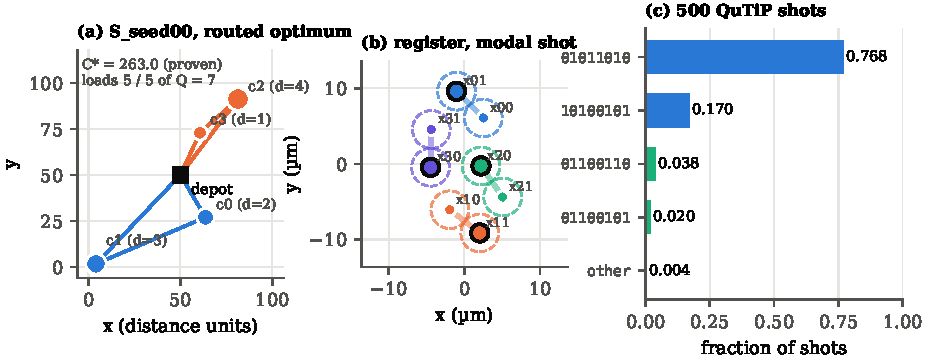
\includegraphics[width=\textwidth]{fig1_pipeline.pdf}
\caption{The pipeline on the headline instance. (a) S\_seed00 with its proven-optimal clustering, routed exactly ($C^*=263.0$). (b) The 8-atom register: four 5\,\textmu m dimers, one per customer; bold atoms are excited in the most frequent shot \code{01011010}, which decodes to that clustering. (c) 500 QuTiP shots: the two labelings of the optimal clustering (blue) make up 93.8\,\% of shots; 99.8\,\% are capacity-feasible.}
\label{fig:pipe}
\end{figure*}

\begin{figure*}[t]\centering
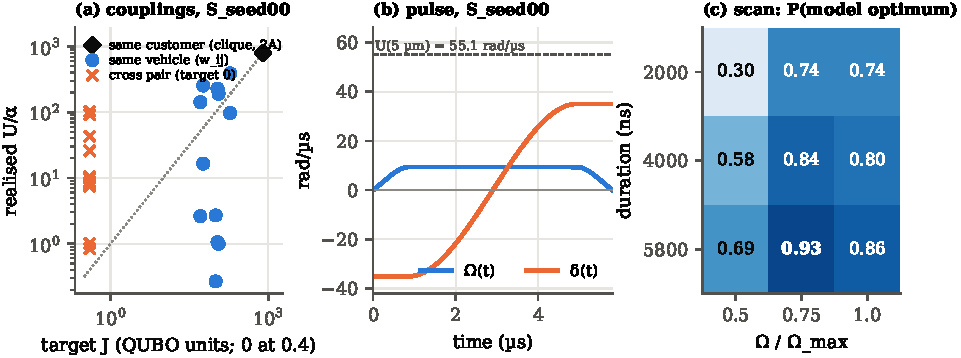
\includegraphics[width=\textwidth]{fig2_embedding_pulse.pdf}
\caption{Embedding and pulse on S\_seed00. (a) Target vs realised couplings by pair class: cliques are exact, same-vehicle couplings approximate, and cross pairs (target 0) are large but nearly constant on valid strings, which is all the model needs. (b) The committed pulse: three-point $\Omega$ ramp at $0.75\,\Omega_{\max}$ and a linear $\delta$ sweep to the fitted $+35.1$\,rad/\textmu s over 5800\,ns, below the 55.1\,rad/\textmu s clique bound. (c) The duration $\times$ amplitude scan (mean over S\_seed00/01/04).}
\label{fig:emb}
\end{figure*}

\section{Pulse (A4)}
We use the baseline of brief Sec.~8.2: a three-point $\Omega$ ramp (15\,\% up, 70\,\% plateau, 15\,\% down) and a linear $\delta$ sweep during the plateau from far below resonance to the fitted $\delta_f$. Every sequence is built with Pulser on \code{AnalogDevice}, serialised, and validated against the device object. We scanned duration and amplitude on three S instances and scored each setting by the probability of reaching the optimum, the best gap and feasibility, never the mean cost (Fig.~\ref{fig:emb}c). Longer was always better, and $0.75\,\Omega_{\max}$ beat full power, which disturbs the 55\,rad/\textmu s cliques more. We committed $T=5800$\,ns and $\Omega=0.75\,\Omega_{\max}$; rescaling $\delta_f$ by 0.8 or 1.25 was worse. Two instances that were not in the scan (S\_seed02/03) reach the optimum in 99\,\% and 96\,\% of shots. Emulators: QuTiP for every tier-S headline row, cross-checked by emu-sv and an in-house exact state-vector integrator; emu-mps for M and L, with bond dimension $\chi$ and peak $\chi$ recorded on every row.

\begin{table*}[t]\centering\footnotesize
\caption{The improvement ladder. Each step was measured on the same instances and committed registers before and after the change (raw shots, 500 per row, no repair). P(opt) = fraction of shots that are the model-optimal clustering. Values are per instance in the order listed.}
\setlength{\tabcolsep}{4pt}\renewcommand{\arraystretch}{1.12}
\begin{tabularx}{\textwidth}{@{}c>{\raggedright\arraybackslash}p{3.6cm}Yp{2.2cm}>{\raggedright\arraybackslash}p{5.0cm}@{}}\toprule
\# & What we changed & Why & Measured on & Before $\to$ after \\\midrule
1 & Textbook slack $\to$ one-hot + unbalanced penalization & Slack bits cost atoms and give non-uniform linear terms that a global detuning cannot realise & all tiers & Atoms 14/45/80 $\to$ \textbf{8/30/60}; linear terms non-uniform $\to$ uniform \\
2 & Generic embedder $\to$ polygons fitted on one-hot subspace & ``Zero'' cross couplings came out as strong as the wanted ones & S\_seed00/01/04 & Coupling error 0.95 $\to$ 0.21--0.32; P(opt) 0.13/0.07/0.03 $\to$ \textbf{0.90/0.88/0.62}; feasibility 0.22/0.09/0.06 $\to$ 0.99/0.88/0.99 \\
3 & Pulse 4000\,ns at $\Omega_{\max}$ $\to$ 5800\,ns at $0.75\,\Omega_{\max}$ & Longer sweep; gentler drive on the clique couplings & S\_seed00/01/04 & P(opt) 0.90/0.88/0.62 $\to$ \textbf{0.94/0.95/0.89}; feasibility 0.99/0.88/0.99 $\to$ 1.00/0.95/1.00 \\
4 & Enforce $\delta_f<U_{\rm clique}$ & Fit ran to 125.66\,rad/\textmu s, rewarding two excitations per triangle & M\_seed00/02 & Decodable 0/0 $\to$ \textbf{0.99/1.00}; feasible 0/0 $\to$ 0.044/0.446 \\
5 & Bound from the weakest polygon pair & A square's diagonal coupling is 8$\times$ weaker than its side & tier L & $\delta_f$ 35.8 $\to$ 4.5\,rad/\textmu s; the mis-set run was discarded before reporting \\
6 & 5\,\textmu m $\to$ 8\,\textmu m spacing between polygons & Caps spurious couplings at 3.3\,rad/\textmu s; defect gaps 1.1 $\to$ 2.4\,rad/\textmu s & L\_seed00/01/02 & Optimum's one-hot rank on L\_seed00: 16\,534 $\to$ 1\,795 \\
7 & Drive matched to the $K=4$ energy scale, $\Omega$ $0.75\to0.15\,\Omega_{\max}$ & The whole one-hot landscape spans a few rad/\textmu s & L\_seed00/01/02 & Feasible 0.008/0.004/0 $\to$ \textbf{0.208/0.140/0.226}; best CVRP gap 80/75/--- $\to$ \textbf{47/40/36\,\%} \\
8 & Bond dimension $\chi=32\to64$ & Convergence of the 30-atom emulation & M\_seed01 & Best CVRP gap 9.2 $\to$ \textbf{5.9\,\%}; peak $\chi$ 14 (converged) \\
\bottomrule
\end{tabularx}
\label{tab:ladder}
\end{table*}

\section{Results (A4, brief Table 3)}\label{sec:results}
Table~\ref{tab:ladder} lists every improvement we made, each measured before and after on the same instances. Table~\ref{tab:head} gives the best final row per tier with the metrics the brief asks for; all 79 rows are in \code{results.csv}, one per (instance, method, seed), with atoms, feasibility, best model and CVRP gaps on feasible decodes, P(reach $C^*$), P(gap $\le\varepsilon$) for $\varepsilon\in\{0,1,5,10\}\,\%$ (we quote 5\,\%), fidelity, reference status, $\chi$, DMM (never used) and repair label.

\begin{table*}[t]\centering\footnotesize
\caption{Best final row per tier (brief Table 3 metrics). Raw shots, no repair, no DMM; every gap on feasible decodes only; $\varepsilon=5\,\%$. Fidelity = $\|U/\alpha-J\|_F/\|J\|_F$ on the full matrix (one-hot-subspace value in parentheses).}
\setlength{\tabcolsep}{4pt}\begin{tabular}{@{}llccccccccl@{}}\toprule
instance & method / backend & atoms & feas. & model gap & CVRP gap & P($C^*$) & P(gap$\le$5\,\%) & fidelity & reference & emulation\\\midrule
S\_seed00 & polygons + tuned pulse & 8 & 1.00 & 0.0\,\% & 0.0\,\% & 0.94 & 0.94 & 0.26 (0.38) & proven & QuTiP, exact\\
S\_seed02 & polygons + tuned pulse & 8 & 1.00 & 0.0\,\% & 0.0\,\% & 0.99 & 0.99 & 0.31 (0.28) & proven & QuTiP, exact\\
M\_seed01 & polygons, bounded $\delta_f$ & 30 & 0.39 & 33.8\,\% & 5.9\,\% & 0.00 & 0.00 & 0.08 (0.96) & best known & emu-mps $\chi{=}64$\\
L\_seed02 & 8\,\textmu m polygons, $0.15\,\Omega_{\max}$ & 60 & 0.23 & 47.1\,\% & 36.3\,\% & 0.00 & 0.00 & 0.51 (1.05) & best known & emu-mps $\chi{=}32$\\
\bottomrule
\end{tabular}
\label{tab:head}
\end{table*}

\begin{figure}[t]\centering
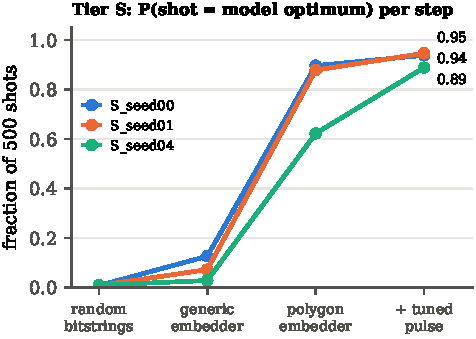
\includegraphics[width=\columnwidth]{fig3_tierS.pdf}
\caption{Tier S, step by step (QuTiP, 500 shots per point; Table~\ref{tab:ladder} rows 2--3). The structure-aware embedder is the largest single gain; the pulse scan closes most of the remaining gap, most of all on S\_seed04.}
\label{fig:S}
\end{figure}

\textbf{Tier S.} On all five instances the register returns the model-optimal clustering in \textbf{0.94/0.95/0.99/0.96/0.89} of raw shots, with feasibility 0.95--1.00 and a 0\,\% model gap (Figs.~\ref{fig:pipe}, \ref{fig:S}). The CVRP gap is 0\,\% on S\_seed00/01/02. On S\_seed03/04 it is 15.6/21.7\,\% while the model gap stays at 0\,\%: the register found the closest clustering, which is not the shortest-route one. That loss is the decomposition gap, and it is a property of the objective, not of the sampler. For context (brief Sec.~9.2), random bitstrings reach the optimum in about 1\,\% of shots, uniformly random valid assignments in 12.5\,\%, and Pasqal's \code{qubo-solver} pipeline in 0--79\,\%. \emph{One ablation shaped the design:} the tighter provable penalty $A=R_w/K$ keeps the optimum as the ground state but drops P(opt) from 0.94 to 0.03 on S\_seed00, because it shrinks the energy margin the sweep needs. We therefore kept the larger $A$.

\textbf{Tier M (30 atoms).} After the $\delta_f$ bound (ladder step 4), 98--100\,\% of shots are one-hot and 4.4/38.8/44.6\,\% are capacity-feasible. The best CVRP gaps are 29.9/5.9/16.0\,\% (M\_seed01 at $\chi=64$). Enumerating all $3^{10}$ one-hot strings shows where the remaining loss sits: the capacity term costs nothing on two instances, and the pulse is not the bottleneck, because the sampled best shots beat the register's own best feasible one-hot string. The loss is the register's ordering of clusterings (the optimum sits at rank 4\,192--12\,966 of 59\,049), the geometric limit of $K=3$ triangles.

\begin{figure*}[t]\centering
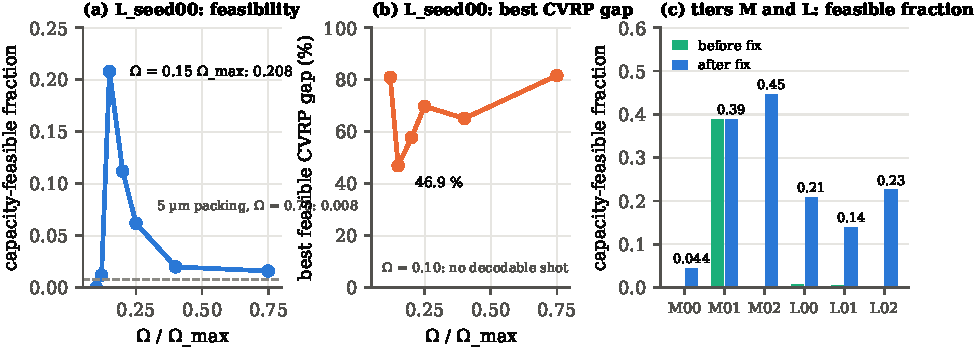
\includegraphics[width=\textwidth]{fig4_tierML.pdf}
\caption{Tiers M and L (emu-mps $\chi=32$, 500 shots). (a,b) L\_seed00 at 8\,\textmu m polygon spacing: matching the drive to the compressed $K=4$ energy scale ($\Omega=0.15\,\Omega_{\max}=1.9$\,rad/\textmu s against 2.4\,rad/\textmu s defect gaps) is a sharp optimum. It moves L\_seed00 from 0.8\,\% feasible with an 80\,\% best CVRP gap (5\,\textmu m packing, tier-S drive) to 20.8\,\% and 47\,\%. (c) Capacity-feasible fraction before and after the fixes (M: ladder step 4; L: steps 6--7).}
\label{fig:ML}
\end{figure*}

\textbf{Tier L (60 atoms, $K=4$).} The weak square diagonal caps $\delta_f$ at 4.5\,rad/\textmu s and squeezes the whole one-hot landscape into a few rad/\textmu s. With the 5\,\textmu m packing and the tier-S drive, only 0.8/0.4/0\,\% of shots were feasible. Spacing the polygons to 8\,\textmu m and matching $\Omega$ to the new energy scale (ladder steps 6--7, Fig.~\ref{fig:ML}) raised feasibility to \textbf{20.8/14.0/22.6\,\%} and brought the best CVRP gaps to \textbf{46.9/40.4/36.3\,\%}, with 37--41\,\% of shots one-hot. The amplitude is a sharp optimum: at $0.10\,\Omega_{\max}$ no shot decodes, and above $0.25$ performance falls off again. Emulation: emu-mps, $\chi=32$, d$t$=10\,ns, precision $10^{-5}$, peak $\chi$ 17--32.

\textbf{Follow-up studies.} Decomposition gaps are 0/0/0/15.6/21.7\,\% (S), 0/0/6.9\,\% (M) and 17.6/8.2/13.1\,\% (L). An exact comparison of three clustering objectives shows that a depot-aware one, $\mathrm{MST}(S)+2\min_{i\in S}d_{0i}$, cuts the L decomposition gaps to 0/0/7.5\,\% but worsens every M instance; it is the natural next objective for L. On eight deliberately capacity-binding S instances (four held out, selection frozen first), a stronger balance weight $\kappa=0.6$ raises mean feasibility from 0.48 to 0.80 but lowers mean P(reach $C^*$) from 0.39 to 0.19, so it stays an ablation. A bounded classical repair makes 98--100\,\% of M shots feasible; it is reported separately and never mixed into raw metrics.

\section{Track B: routing (B1--B3)}
\textbf{B1.} For a cluster of $n$ customers plus the depot, $y_{i,t}=1$ if customer $i$ is visited at position $t$. The objective is $\sum_t\sum_{i\ne j}c_{ij}y_{i,t}y_{j,t+1}$ plus the two depot legs; each customer takes one position and each position one customer (both equalities).
\textbf{B2, two encodings.} (i) \emph{Depot-fixed position}, $n^2$ bits. The depot gets no variables; its legs are folded into the first and last transition weights, $w(i,j,t)=c_{ij}+[t{=}1]c_{0i}+[t{=}n-1]c_{j0}$. The energy then equals the tour length exactly on every valid string, and every linear term is $-2A$. This saves $2n+1$ bits over the textbook $(n+1)^2$. (ii) \emph{Undirected edge}, $n(n+1)/2$ bits: one bit per edge, a degree-2 penalty, and each edge's cost split between its two endpoints so the linear terms stay uniform ($-6A$). It is exact for $n\le4$; for $n\ge5$ two disjoint triangles can be cheaper than any tour, which we demonstrate explicitly. Both encodings were verified by exhaustive enumeration on 18 cases (Fig.~\ref{fig:B}a).
\textbf{B3.} Clusters with $n\le3$ are trivial and routed exactly; $n=4$ clusters run both encodings (10 and 16 atoms, exact state-vector emulation, 1000 shots each); $n\ge5$ are routed classically and labelled. On the tier-M clusterings, 12 clusters were routed: 7 trivial, 5 quantum attempts, one raw valid quantum tour (20.4\,\% routing gap) and 4 labelled classical fallbacks, so 1 of 5 non-trivial clusters was routed quantumly. End-to-end gaps are 19.6\,\% (M\_seed01) and 16.0\,\% (M\_seed02), split exactly into decomposition, clustering and routing loss (Fig.~\ref{fig:B}b). Both routing QUBOs are correct; the limit is the generic embedding, and a structure-aware routing register, built the same way as Track A's, is the next step.

\begin{figure*}[t]\centering
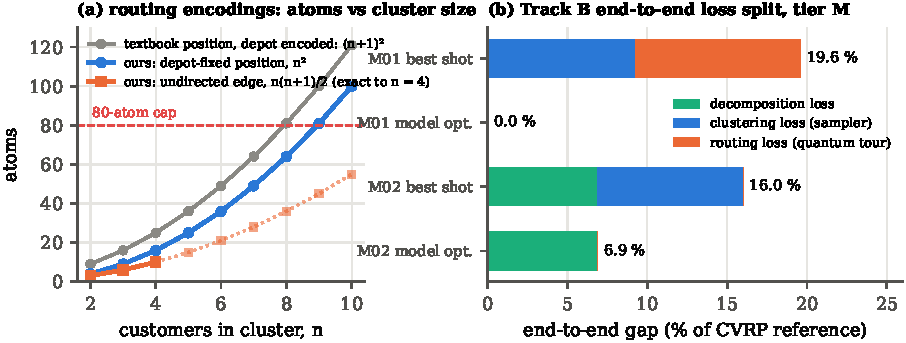
\includegraphics[width=0.92\textwidth]{fig5_trackB.pdf}
\caption{Track B. (a) Atoms needed by each routing encoding as the cluster grows; the edge model is exact up to $n=4$. (b) End-to-end loss split into decomposition + clustering + routing, an identity verified to $10^{-9}$ on every row.}
\label{fig:B}
\end{figure*}

\section{What did not work}
\begin{itemize}
\item \textbf{Generic embedding of the coupling graph:} error 0.95, P(opt) 3--13\,\%, and an infeasible ground state on S\_seed04. Fixed for $K=2$ by the polygon fit; for $K\ge3$ the ordering of clusterings is still distorted.
\item \textbf{Unbounded $\delta_f$ on tier M:} 0 of 500 shots decodable on two instances. The first L run, set with the triangle bound, would have favoured two opposite corners and was discarded.
\item \textbf{No single $\kappa$ works on all toy seeds} (best 35/40): where capacity binds, ``closest'' and ``most balanced'' conflict, and a soft term cannot force $L_k\le Q$.
\item \textbf{The weight scan showed no trend}, because the embedding optimiser lands in a different local minimum each time. It is also not bit-identical across platforms (51\,\% vs 90\,\% from one seed), so every register is committed.
\item \textbf{The tight $A$} is provably sound but removes the device's margin (0.94 $\to$ 0.03).
\item \textbf{qubo-solver's annealer} returned the same non-optimal string on three S instances, and its uncapped emu-mps run on M ($\chi>300$) was stopped after 80\,min.
\item \textbf{Track B:} one valid quantum tour in 10\,000 shots with the generic embedding.
\item \textbf{Plumbing:} no CPLEX wheel; a cp1252 console crash on ``$\delta$''; a \code{|} in a file name lost a record on Windows; a stale PDF was briefly reported as fresh; a sync reset a parallel edit. All are fixed and logged in \code{docs/DID\_NOT\_WORK.md}.
\end{itemize}

\section{Conclusions and next steps}
We showed that the capacity inequality can go onto an analog register with \emph{zero} slack atoms, all couplings positive and one global detuning, at $NK$ atoms on every tier. Each step from paper to device was measured: the polygon embedder and the pulse scan took tier S to 89--99\,\% optimal shots; a derived detuning bound made tier M decodable; and a register and drive matched to the $K=4$ energy scale took tier L from under 1\,\% to 14--23\,\% feasible shots. The next improvements are in the register: an encoding of ``which vehicle'' that avoids $K$-gons (for example hierarchical $K=2$ bisection, which keeps every tier-S property), a depot-aware objective for L, and a structure-aware routing register for Track B.

\noindent\textbf{Use of AI.} Claude and Codex were used throughout: typing up and, at the team's request, drafting derivations, and writing code, scans, figures, tables and prose. A fresh-context AI reviewer audited physics, algebra and fairness. Every number here is generated from run records; algebra is checked by exhaustive tier-S enumeration and device legality by Pulser. The team chose the model, the protocol and the claims, and owns all of them (\code{docs/AI\_USE.md}).

\begin{thebibliography}{9}\small
\bibitem{montanez} J.~A. Monta\~nez-Barrera, D.~Willsch, A.~Maldonado-Romo, K.~Michielsen, \emph{Unbalanced penalization: a new approach to encode inequality constraints of combinatorial problems for quantum optimization algorithms}, Quantum Sci. Technol. 9, 025022 (2024), arXiv:2211.13914.
\end{thebibliography}
\end{document}
